\section{Evaluasi Eksperimen}

Model dilatih sesuai dengan konfigurasi yang telah disebutkan pada subbab \ref{sec:pelatihan-model} dan dilatih pada lingkungan eksperimen yang telah disebutkan pada subbab \ref{sec:lingkungan-eksperimen}. Eksperimen dilakukan pada setiap tugas evaluasi yaitu \nlptask. Setiap tugas evaluasi dilatih dengan \textit{fine-tuning}, \methodPEFT. Hasil evaluasi dilakukan pada 5-\textit{fold} dengan setiap evaluasi terdapat nilai rata-rata, minimum, dan maksimum dari \textit{fold} tersebut.

\subsection{Hasil Evaluasi NER}
\label{sec:ner-evaluation}

Evaluasi dilakukan untuk model IndoBERT dengan melakukan 8 eksperimen (\textit{fine-tuning} dan PEFT beserta variasinya) pada 5-\textit{fold dataset} NER UI dan NER UGM. Hasil evaluasi yang didapatkan yaitu waktu pelatihan dan skor F1 dari data evaluasi yang bisa dilihat pada tabel \ref{table:runtime-ner} dan gambar \ref{fig:ner-result}. Skor F1 didapatkan dari \textit{weighted} F1 terhadap level entitas. Skor F1 dan waktu pelatihan merupakan hasil dari rata-rata pada seluruh 5-\textit{fold}.

\begin{table}[h]
    \centering
    \caption{Waktu pelatihan tugas NER}
    \label{table:runtime-ner}
    \begin{tabular}{l|r|r}
        \toprule
        \textbf{Metode} & \textbf{Waktu(s) NER UI} & \textbf{Waktu(s) NER UGM} \\
        \midrule
        \textit{Fine-tuning} & 884 (100\%) & 974 (100\%) \\
        LoRA ($r$=8) & 528 (60\%) & 580 (60\%) \\
        LoRA ($r$=16) & 515 (58\%) & 588 (60\%) \\
        Prefix Tuning ($pl$=5) & \textcolor{Green}{494 (56\%)} & \textcolor{Green}{562 (58\%)} \\
        Prefix Tuning ($pl$=50) & 534 (60\%) & 598 (61\%) \\
        Adapter ($rf$=64) & 564 (64\%) & 587 (60\%) \\
        Adapter ($rf$=16) & 563 (64\%) & 595 (61\%) \\
        UniPELT & \textcolor{Red}{928 (105\%)} & \textcolor{Red}{991 (102\%)} \\
        \bottomrule
    \end{tabular}
\end{table}

Berdasarkan waktu pelatihan yang bisa dilihat pada tabel \ref{table:runtime-ner}, didapatkan bahwa terdapat peningkatan (lebih cepat) dibandingkan dengan metode \textit{fine-tuning}. Dengan waktu pelatihan yang paling cepat adalah untuk metode \textit{Prefix-Tuning} $pl=5$ untuk kedua \textit{dataset} dengan waktu pelatihan selama 494 detik dibandingkan 884 detik (\textit{fine-tuning}) yang menggunakan 56\% waktu pelatihan untuk NER UI dan 58\% untuk NER UGM. Sedangkan, pada UniPELT didapatkan hasil yang lebih buruk bahkan ketika dibandingkan dengan \textit{fine-tuning} dengan waktu 928 detik, ketika dibandingkan dengan \textit{fine-tuning}, hasilnya memburuk dengan 102\% waktu pelatihan. Selain itu, untuk metode PEFT yang lainnya mempunyai hasil yang konsiten jika dibandingkan dari penelitian yang dilakukan oleh \citeauthor{unipelt}, dengan setiap banya menggunakan sekitar 56\% sampai 64\%, terkecuali pada UniPELT.

\begin{figure}[h]
    \centering
    \centerline{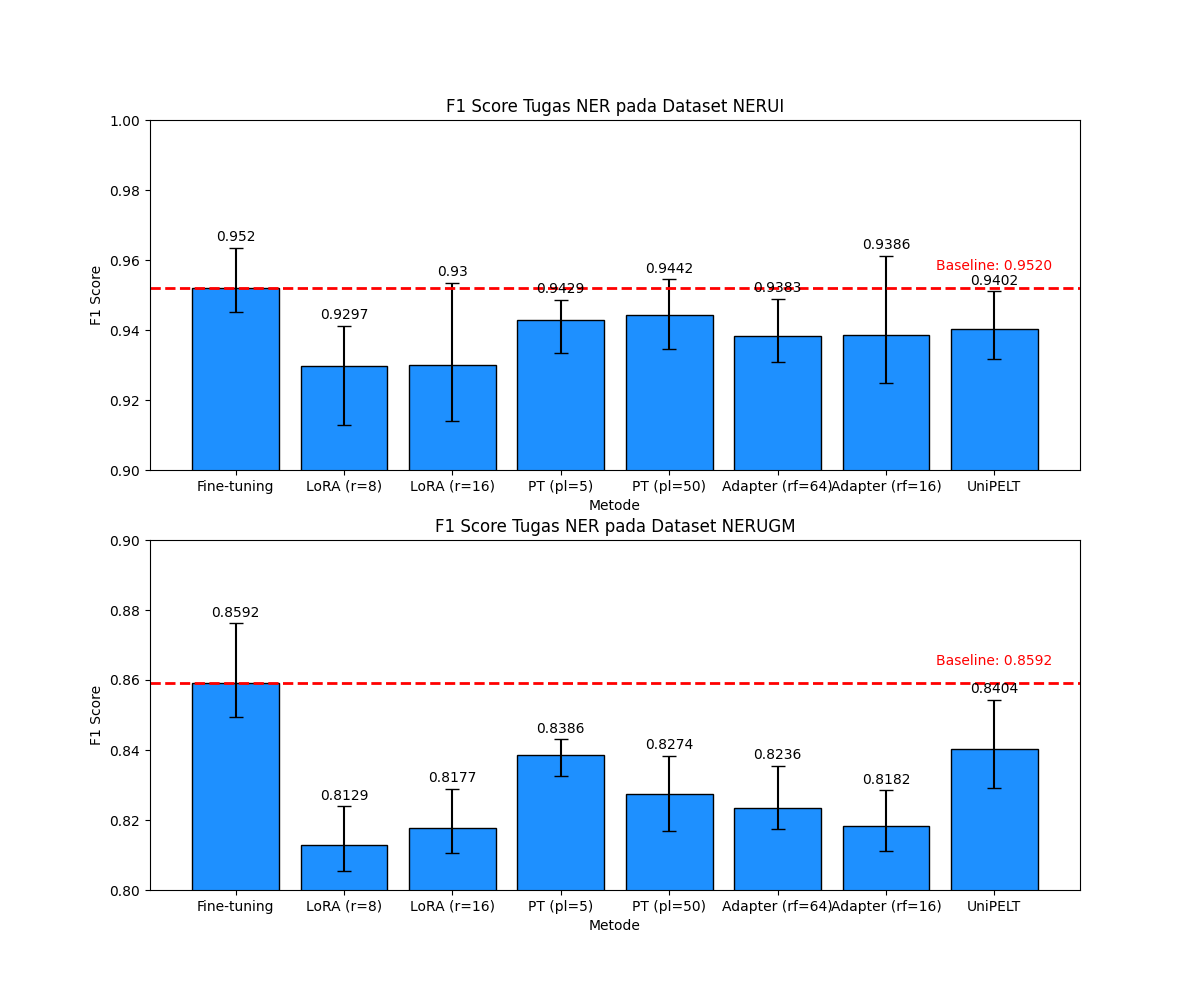
\includegraphics[width=1.2\textwidth]{chapter-4/ner_result.png}}
    \caption{\textit{F1 Score} Hasil Evaluasi NER}
    \label{fig:ner-result}
\end{figure}

Dari gambar \ref{fig:ner-result} didapatkan hasil evaluasi F1 skor terhadap kedua \textit{dataset}, yaitu NER UI (atas) dan NER UGM (bawah). Didapatkan skor F1 untuk \textit{fine-tuning} adalah 0,952 (NER UI) dan 0,859 (NER UGM). Untuk metode PEFT, hasil yang paling mendekati adalah \textit{Prefix-Tuning} $pl=50$ dengan skor F1-nya bernilai 0,944 (NER UI) dan UniPELT dengan skor F1-nya 0,84 (NER UGM). Perbandingan untuk \textit{dataset} NER UI antara \textit{fine-tuning} dengan PEFT terbaik (dalam konteks ini \textit{Prefix-Tuning} $pl=50$) adalah 0,952 dibanding 0,944, dengan selisih sebanyak 0,008 yang berati terdapat perbedaan sebanyak 0,84\%. Lalu, perbandingan untuk NER UGM adalah 0,859 dibanding 0,84, dengan selisih sebanyak 0,0188 yang berarti terdapat perbedaan sebanyak 2,2\%. 

Metode PEFT yang terburuk pada tugas evaluasi ini adalah LoRA $r=8$ dengan nilai 0,923 untuk NER UI dan 0,813 untuk NER UGM. Ketika dibandingkan dengan \textit{fine-tuning}, untuk NER UI adalah 0,952 dibanding 0,923 dengan selisih sebesar 3\%. Lalu, untuk NER UGM, nilainya adalah 0,859 dibanding 0,813 dengan selisih 5,4\%. Ketika ditinjau sebagai rentang persentase selisih secara keseluruhan, didapatkan rentang antara 0,84\% sampai 5,4\% untuk tugas evaluasi NER. Perbandingan yang cukup kecil mengingat dari jumlah parameter yang digunakan dan waktu pelatihannya yang lebih singkat.

Ditinjau dari konfigurasi model PEFT yang digunakan, pada hal ini adalah $rank$ untuk LoRA, $prefix\_length$ untuk \textit{Prefix-Tuning}, dan $reduction\_factor$ untuk \textit{Adapter}, hanya LoRA yang konsisten lebih baik pada kedua \textit{dataset}. \textit{Prefix-Tuning} dan \textit{Adapter} tidak konsisten berdasarkan konfigurasi pada hasil evaluasi. Untuk meninjau kinerja setiap PEFT secara setara dilakukan perbandingan dengan menggunakan konfigurasi yang terbaik untuk setiap \textit{dataset} yang bisa dilihat pada tabel \ref{table:ner-result-desc}.

\begin{table}[h]
    \centering
    \caption{Tabel skor F1 (terurut secara menurun) tugas NER dengan konfigurasi terbaik}
    \label{table:ner-result-desc}
    \begin{tabular}{ll|ll}
        \toprule
        \textbf{Metode} & \textbf{F1 NER UI $\downarrow$} & \textbf{Metode} & \textbf{F1 NER UGM $\downarrow$} \\
        \midrule
        \textit{Fine-tuning} & 0,952 & \textit{Fine-tuning} & 0,859 \\
        \textit{Prefix-Tuning} & 0,944 & UniPELT & 0,84 \\
        \textit{UniPELT} & 0,94 & \textit{Prefix-Tuning} & 0,838 \\
        \textit{Adapter} & 0,939 & \textit{Adapter} & 0,824 \\
        LoRA & 0,93 & LoRA & 0,82 \\
        \bottomrule
    \end{tabular}
\end{table}

Hasil yang didapatkan dengan menggunakan konfigurasi metode PEFT terbaik dan diurutkan secara menurun bisa dilihat pada tabel \ref{table:ner-result-desc}. Berdasarkan hasil tersebut, \textit{fine-tuning} tetap mendapatkan hasil yang terbaik, disusul oleh \textit{UniPELT} dan \textit{Prefix-Tuning} pada peringkat yang sama, \textit{Adapter}, dan LoRA pada urutan terakhir.

\subsection{Hasil Evaluasi \textit{Sentiment Analysis}}
\label{sec:sentiment-evaluation}

Evaluasi dilakukan untuk model IndoBERT dengan melakukan 8 eksperimen (\textit{fine-tuning} dan PEFT beserta variasinya) pada 5-\textit{fold dataset} untuk tugas \textit{sentiment analysis}. Berbeda dengan tugas NER yang dibahas pada subbab \ref{sec:ner-evaluation}, tugas \textit{sentiment analysis} hanya mempunyai satu \textit{dataset} yang tersedia pada kakas evaluasi IndoLEM. Hasil evaluasi yang didapatkan merupakan waktu pelatihan dan juga skor F1 dari data evaluasi, hasil tersebut bisa dilihat pada tabel \ref{table:runtime-sentiment} dan gambar \ref{fig:ner-result}. Sama seperti subbab \ref{sec:ner-evaluation}, skor F1 dan waktu pelatihan merupakan hasil dari rata-rata pada seluruh 5-\textit{fold}.

\begin{table}[h]
    \centering
    \caption{Waktu pelatihan tugas \textit{sentiment analysis}}
    \label{table:runtime-sentiment}
    \begin{tabular}{l|rr}
        \toprule
        \textbf{Metode} & \textbf{Waktu(s) \%} \\
        \midrule
        \textit{Fine-tuning} & \textcolor{Red}{866 (100\%)} \\
        LoRA ($r$=8) & 627 (72\%) \\
        LoRA ($r$=16) & 627 (72\%) \\
        Prefix Tuning ($pl$=5) & 619 (72\%) \\
        Prefix Tuning ($pl$=50) & 652 (75\%) \\
        Adapter ($rf$=64) & \textcolor{Green}{613 (71\%)} \\
        Adapter ($rf$=16) & 617 (71\%) \\
        UniPELT & 746 (86\%) \\
        \bottomrule
    \end{tabular}
\end{table}

Dari tabel \ref{table:runtime-sentiment}, didapatkan waktu pelatihan yang paling cepat adalah \textit{Adapter} $rf=64$ dengan waktu yang dibutuhkan sebanyak 613 detik, sebaliknya waktu pelatihan yang paling lambat adalah \textit{fine-tuning} dengan waktu sebesar 866 detik. Perbandingan antara waktu pelatihan yang tercepat yaitu \textit{Adapter} $rf=64$ dengan perbandingan sebesar 71\% dibandingkan dengan waktu pelatihan pada \textit{fine-tuning}. Untuk tugas evaluasi \textit{sentiment analysis}, setiap metode PEFT berhasil mendapatkan waktu pelatihan yang lebih cepat dibandingkan dengan \textit{fine-tuning}. Rentang perbandingan waktu yang dibutuhkan dibandingkan dengan \textit{fine-tuning} adalah antara 71\% (\textit{Adapter}) sampai 86\% (UniPELT). Rasio dari waktu pelatihan yang didapatkan sesuai dengan pada penelitian yang dilakukan oleh \citeauthor{unipelt}, bisa dilihat pada tabel \ref{table:unipelt_result}.

\begin{figure}[h]
    \centering
    \centerline{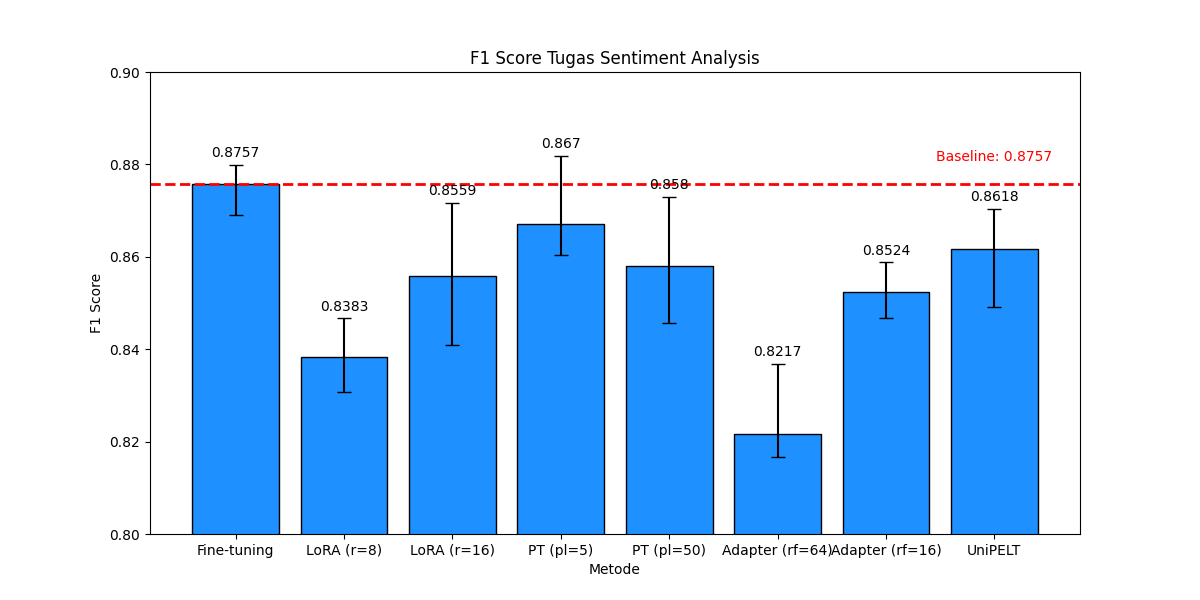
\includegraphics[width=1.2\textwidth]{chapter-4/sentiment_result.png}}
    \caption{\textit{F1 Score} Hasil Evaluasi \textit{Sentiment Analysis}}
    \label{fig:sentiment-result}
\end{figure}

Berdasarkan skor F1 pada gambar \ref{fig:sentiment-result}, \textit{fine-tuning} mendapatkan skor yang terbaik dengan nilai 0,876 disusul oleh metode \textit{Prefix-Tuning} $pl=5$ dengan nilai 0,867. Selisih yang didapatkan antara \textit{fine-tuning} dengan metode PEFT terbaik (\textit{Prefix-Tuning} $pl=5$) adalah 0,876 dibanding 0,867, dengan nilai selisihnya yaitu 0,009 atau sekitar 1\%. Sedangkan, untuk metode PEFT terburuk secara skor F1 adalah 0,822 yaitu metode \textit{Adapter} $rf=64$. Dibandingkan antara \textit{fine-tuning} dengan \textit{Adapter} $rf=64$ yaitu 0,822 dibanding 0,876 dengan selisihnya sebesar 0,054 atau sekitar 6,2\%. Demikian didapatkan rentang selisih untuk semua metode PEFT dibandingkan dengan \textit{fine-tuning} adalah antara 1\% sampai 6,2\%. Perbandingan ini terhitung cukup kecil jika mengingat penggunaan parameter pelatihan dan waktu pelatihan yang lebih sedikit. Sehingga, terdapat \textit{tradeoff} antara parameter pelatihan yang lebih kecil dan waktu pelatihan yang lebih cepat dengan hasil evaluasi yang lebih buruk.

Pada tugas evaluasi ini, konfigurasi untuk metode PEFT konsisten lebih baik untuk parameter yang lebih banyak untuk LoRA dan \textit{Adapter}. LoRA dengan $r=16$ mendapatkan hasil yang lebih baik dibandingkan dengan $r=8$. Begitu juga dengan \textit{Adapter} dengan $rf=16$ mendapatkan hasil yang lebih baik dibanding $rf=64$ ($rf$ merupakan faktor reduksi, sehingga $rf$ yang lebih kecil akan menghasilkan parameter yang lebih banyak). Tetapi, hal yang sebaliknya terjadi untuk metode \textit{Prefix-Tuning}, variasi $pl=5$ ternyata menghasilkan skor F1 yang lebih baik dibandingkan dengan $pl=50$. Untuk meninjau kinerja metode PEFT secara dilakukan perbandingan dengan skor F1 berdasarkan hasil yang paling baik untuk setiap variasinya.

\begin{table}[h]
    \centering
    \caption{Tabel F1 (terurut secara menurun) tugas \textit{sentiment analysis} dengan konfigurasi terbaik}
    \label{table:sentiment-result-desc}
    \begin{tabular}{l|l}
        \toprule
        \textbf{Metode} & \textbf{F1 $\downarrow$} \\
        \midrule
        \textit{Fine-tuning} & 0,876 \\
        \textit{Prefix-tuning} & 0,867 \\
        \textit{UniPELT} & 0,862 \\
        \textit{LoRA} & 0,856 \\
        \textit{Adapter} & 0,852 \\
        \bottomrule
    \end{tabular}
\end{table}

Tabel \ref{table:sentiment-result-desc} menunjukkan skor F1 yang terurut secara menurun untuk metode PEFT dengan konfigurasi terbaik. \textit{Fine-tuning} mendapatkan hasil yang paling baik, disusul oleh \textit{Prefix-Tuning}, UniPELT, LoRA, lalu Adapter. Urutan ini cukup konsisten dengan untuk tugas NER pada tabel \ref{table:ner-result-desc}. Namun, terdapat perbedaan untuk metode PEFT pada urutan terakhir, pada tugas evaluasi ini, urutan terakhir dipegang oleh \textit{Adapter}.

\subsection{Hasil Evaluasi \textit{Summarization}}

Evaluasi dilakukan untuk model IndoT5 dengan melakukan 8 eksperimen (\textit{fine-tuning} dan PEFT beserta variasinya) pada \textit{dataset} IndoSum yang tersedia pada kakas IndoLEM. Meskipun \textit{dataset} untuk tugas \textit{summarization} menggunakan 5-\text{fold cross validation}, tetapi pada eksperimen ini tidak dilakukan untuk 5\textit{-fold}, hanya dilakukan pada \textit{fold} pertama saja karena kerterbatasan sumber daya. Hasil evaluasi yang didapatkan berupa waktu pelatihan dan skor ROUGE (R1, R2, dan RL) dari data evaluasi, hasil tersebut bisa dilihat pada tabel \ref{table:runtime-summarization-indosum} dan gambar \ref{fig:summarization-result-indosum}.

\begin{table}[h]
    \centering
    \caption{Waktu pelatihan tugas \textit{summarization} IndoSum}
    \label{table:runtime-summarization-indosum}
    \begin{tabular}{l|r}
        \toprule
        \textbf{Metode} & \textbf{Waktu(s) \%} \\
        \midrule
        \textit{Fine-tuning} & 5026 (100\%) \\
        LoRA ($r$=8) & 4841 (96\%) \\
        LoRA ($r$=16) & 4900 (97\%) \\
        Prefix Tuning ($pl$=5) & 6618 (132\%) \\
        Prefix Tuning ($pl$=50) & \textcolor{Red}{11379 (227\%)} \\
        Adapter ($factor$=64) & \textcolor{Green}{4578 (91\%)} \\
        Adapter ($factor$=16) & 4587 (91\%) \\
        UniPELT & 9241 (184\%) \\
        \bottomrule
    \end{tabular}
\end{table}

Dari waktu pelatihan yang didapatkan dari tabel \ref{table:runtime-summarization-indosum}, terdapat waktu pelatihan tercepat adalah \textit{Adapter} $rf=64$ dengan waktu sebesar 4,578 detik. Untuk waktu pelatihan yang terlambat adalah \textit{Prefix-Tuning} $pl=50$ dengan waktu sebesar 11,379 detik. Jika dibandingkan dengan \textit{fine-tuning}, waktu tercepat menggunakan 91\% dari waktu pelatihan, hal ini berbeda dari subbab \ref{sec:ner-evaluation} dan \ref{sec:sentiment-evaluation} yang bisa mendapatkan hasil lebih cepat. Selain itu, untuk waktupaling lambat didapatkan perbandingan sebesar 227\%, yang berarti waktu pelatihannya lebih dari 2 kali lipat dibanding \textit{fine-tuning}. Metode \textit{Prefix-Tuning} dan UniPELT membutuhkan waktu pelatihan yang lebih dari \textit{fine-tuning} ($>100\%$). 

Untuk memastikan perilaku ini konsisten terhadap tugas \textit{summarization}, dilakukan percobaan pada metode \textit{Prefix-Tuning} pada \textit{fold} yang berbeda. Untuk \textit{fold} yang berbeda juga didapatkan hasil yang sama, yaitu 6535 detik untuk $pl=5$ pada \textit{fold} kedua. Perilaku ini konsisten terhadap tugas \textit{summarization} pada \textit{dataset} IndoSum. Dilakukan juga eksperimen pada \textit{dataset} yang berbeda, yaitu Liputan6 secara \textit{abstractive} dan \textit{extractive}. Untuk mempersingkat eksperimen yang dilakukan, hanya digunakan sampel data sebanyak 1000 untuk setiap data latih, validasi, dan uji pada Liputan6.

\begin{table}[h]
    \centering
    \caption{Waktu pelatihan tugas \textit{summarization} Liputan6}
    \label{table:runtime-summarization-liputan6}
    \begin{tabular}{l|r|r}
        \toprule
        \multirow{2}{*}{\textbf{Metode}} & \textbf{Waktu(s)}  & \textbf{Waktu(s)}  \\
                                         & \textbf{\textit{Abstractive}} & \textbf{\textit{Extractive}} \\
        \midrule
        \textit{Fine-tuning} & 1412 (100\%) & 1485 (100\%) \\
        LoRA ($r=8$) & 1410 (100\%) & 2125 (143\%) \\
        LoRA ($r=16$) & 1512 (107\%) & 2138 (144\%) \\
        \textit{Prefix-Tuning} ($pl=5$) & 1435 (102\%) & 1610 (108\%) \\
        \textit{Prefix-Tuning} ($pl=50$) & \textcolor{Red}{4252 (301\%)} & \textcolor{Red}{6572 (443\%)} \\
        \textit{Adapter} ($rf=64$) & \textcolor{Green}{727 (51\%)} & 1265 (85\%) \\
        \textit{Adapter} ($rf=16$) & 754 (53\%) & \textcolor{Green}{1217 (82\%)} \\
        UniPELT & 4104 (291\%) & 4145 (279\%) \\
        \bottomrule
    \end{tabular}
\end{table}

Hasil yang sama juga didapatkan dengan \textit{dataset} yang berbeda, seperti yang bisa dilihat pada tabel \ref{table:runtime-summarization-liputan6}. Metode \textit{Prefix-Tuning} perlu menggunakan waktu paling lama, bahkan pada Liputan6 secara \textit{extractive} waktu pelatihan sampai 4 kali lipatnya. Untuk tugas \textit{summarization}, tidak didapatkan hasil yang konsisten antara perbandingan parameter dengan waktu pelatihannya, terutama pada metode \textit{Prefix-Tuning}. Metode LoRA dan \textit{Adapter} cukup konsiten dibandingkan dengan tugas evaluasi sebelumnya, sedangkan UniPELT terkena dampak dari gagalnya metode \textit{Prefix-Tuning}.

\begin{figure}[h]
    \centering
    \centerline{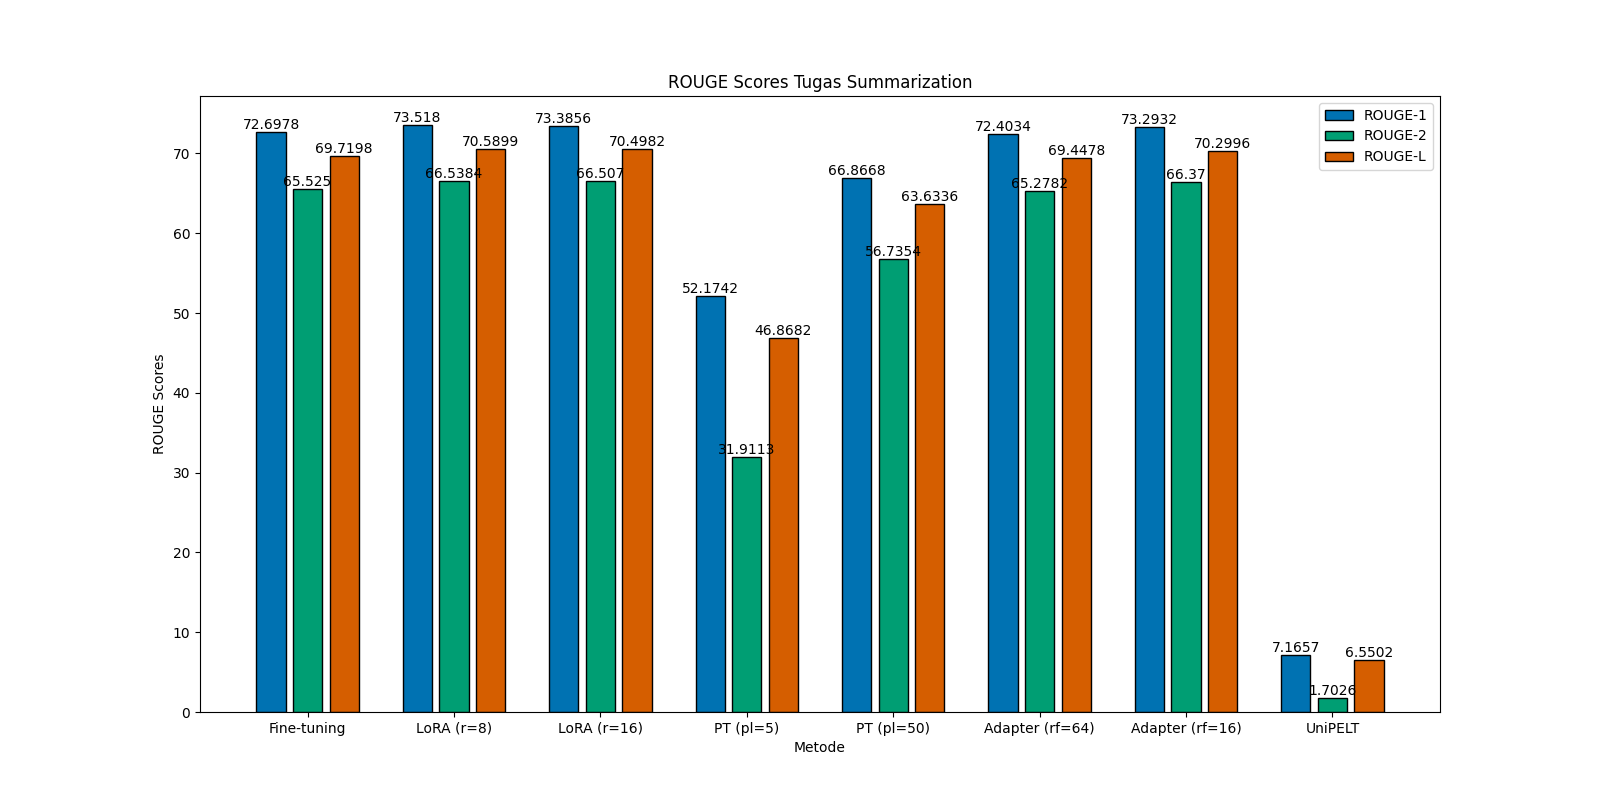
\includegraphics[width=1.4\textwidth]{chapter-4/summarization_result.png}}
    \caption{ROUGE \textit{Score} Hasil Evaluasi \textit{Summarization} pada IndoSum}
    \label{fig:summarization-result-indosum}
\end{figure}

Hasil skor ROUGE untuk \textit{dataset} IndoSum dapat dilihat pada gambar \ref{fig:summarization-result-indosum}. Terdapat tiga skor ROUGE yang digunakan yaitu R1, R2, dan RL. Secara umum, nilai dari R1 adalah yang paling tinggi untuk setiap metode, disusul oleh RL, lalu R2. Hal ini konsisten dengan perhitungan ROUGE yang menggunakan n-gram kecocokan, sehingga R1 yang mencocokan 1-gram kata secara natural akan lebih baik dibanding 2-gram dan L-gram (LCS). Skor ROUGE (ketiganya) yang paling tinggi adalah LoRA $r=8$, ini berbeda dengan tugas evaluasi sebelumnya, yang selalu didahului oleh \textit{fine-tuning}. Sedangkan, untuk nilai yang paling rendah adalah UniPELT degan skor yang sangat buruk.

Selisih yang paling signifikan adalah UniPELT dengan selisih sebesar 90\% dibandingkan dengan \textit{fine-tuning}. Namun, untuk LoRA terdapat peningkatan dengan selisih sebesar +1,25\% (simbol + menandakan peningkatan dari metode \textit{fine-tuning}). Dari selish tersebut, didapatkan rentang kinerja antara metode PEFT dengan \textit{fine-tuning} yaitu dari -90\% sampai +1,25\%. Untuk membandingkan antara metode PEFT secara setara akan dipilih variasi dari setiap PEFT dengan hasil terbaik, hasil perbandingan dapat dilihat pada tabel \ref{table:summarization-result-indosum-desc}.

\begin{table}[h]
    \centering
    \caption{Tabel ROUGE (terurut secara menurun) tugas \textit{summarization} dengan konfigurasi terbaik}
    \label{table:summarization-result-indosum-desc}
    \begin{tabular}{l|lll}
        \toprule
        \textbf{Metode} & \textbf{R1 $\downarrow$} & \textbf{R2 $\downarrow$} & \textbf{RL $\downarrow$} \\
        \midrule
        \textit{LoRA} & 73,52 & 66,54 & 70,59 \\
        \textit{Adapter} & 73,29 & 66,37 & 70,3 \\
        \textit{Fine-tuning} & 72,7 & 65,52 & 69,72 \\
        \textit{Prefix-Tuning} & 66,87 & 56,74 & 63,63 \\
        \textit{UniPELT} & 7,17 & 1,7 & 6,55 \\
        \bottomrule
    \end{tabular}
\end{table}

Berdasarkan tabel \ref{table:summarization-result-indosum-desc}, didapatkan kinerja dari masing-masing metode PEFT yang diurutkan secara menurun. Hasil yang didapatkan sangat berbeda dibanding pada tugas evaluasi NER dan \textit{sentiment analysis}, metode PEFT yaitu LoRA dan \textit{Adapter} unggul dibandingkan dengan \textit{fine-tuning}. Sedangkan, \textit{Prefix-Tuning} dan UniPELT gagal untuk menghasilkan kinerja yang menyaingi \textit{fine-tuning}. UniPELT bahkan hanya menghasilkan perbedaan kinerja sebanyak 90\% lebih buruk.

Sebelumnya, sudah disebutkan pada subbab \ref{sec:prefix-tuning} terkait \textit{Prefix-Tuning} bahwa implementasi dari metode tersebut berbeda karena sudah diadaptasi untuk tugas \textit{classification}. Selain itu, evaluasi yang dilakukan oleh \citeauthor{adapters} (yang mengajukan pustaka Adapters) tidak terdapat tugas evaluasi untuk tugas \textit{generation}. Evaluasi juga menggunakan model RoBERTa yang merupakan variasi dari BERT (\textit{encoder}). Sehingga, memungkinkan bahwa metode \textit{Prefix-Tuning} yang digunakan pada eksperimen ini (tugas \textit{generation} dan model \textit{encoder decoder}) tidak sesuai dengan implementasi dari modul Adapters. Hal ini menyebabkan gagalnya metode \textit{Prefix-Tuning}, yang secara langsung berkaitan juga dengan kegagalan dari UniPELT.
